\section{Balanceo de Par\'entesis}
\subsection{ Descripci\'on del programa}
\justify
El siguiente programa verificar que los par\'entesis de una cadena esten balanceados, el programa tiene un modo manual, la entrada de este modo acepta todo tipo de caracteres ASCII.De igual forma cuenta con un modo autom\'atico con el cual se genera una cadena de par\'entesis aleatoria con una longitud que puede estar entre 0 y 1000.\\
En un archivo se muestra la historia que se sigui\'o al momento de hacer la evualuaci\'on de los par\'entesis, as\'i como las reglas que se utilizaron al momento de evaluar cada car\'acter.\\
\subsection{C\'odigo}
El c\'digo utilizado para la resoluci\'on del problema se muestra a continuaci\'on:\\

C\'odigo:balanceo.py

\lstset{language=Python, breaklines=true, basicstyle=\footnotesize}
\begin{lstlisting}[frame=single]
	

def VerificarBalanceo(cadena,archivo):
    exp='B'
    i=-1;
    cadena_aux=''
    archivo.write(exp)
    while True:
        try:
            i=i+1
            archivo.write('\n')
            if(cadena[i]=='('):
                cadena_aux=cadena_aux+'('
                if(exp[0]=='B'):
                    exp=exp.replace('B','RB',1)
                    cadena_aux=cadena_aux.replace('B','RB',1)
                    archivo.write(cadena_aux+exp)
                    archivo.write('\t\t\tB->(RB')
                    continue
                if(exp[0]=='R'):
                    exp=exp.replace('R','RR',1)
                    cadena_aux=cadena_aux.replace('R','RR',1)
                    archivo.write(cadena_aux+exp)
                    archivo.write('\t\t\tR->(RR')
                    continue
            if(cadena[i]==')'):
                if(exp[0]=='R'):
                    exp=exp[1:]
                    cadena_aux=cadena_aux+')'
                    archivo.write(cadena_aux+exp)
                    archivo.write('\t\t\tR-> )')
                    continue
                elif(exp[0]=='B'):
                    exp=''
                    print('Cadena no balanceada')
                    break
                else:
                    exp=''
                    continue
        except:
            if(exp=='B'):
                archivo.write(cadena_aux)
                archivo.write('\t\t\tB-> e \n')
                print('Cadena balanceada')
            else:
                print('Cadena no balanceada')
            break

\end{lstlisting}
\vspace{1.5cm}
C\'odigo:main.py

\lstset{language=Python, breaklines=true, basicstyle=\footnotesize}
\begin{lstlisting}[frame=single]
	import random
import balanceo

def IniciarArchivo():
    archivo=open("Gramatica.txt","w")
    archivo.close
def Menu():
    print("------Menu-----")
    print("1.-Modo Manual")
    print("2.-Modo Automatico")
    print("3.-Salir")
def Eleccion():
    op=input("Elige una opcion: ")
    try:
        op=int(op)
    except:
        print("Introduzca una opcion valida")
    return op
def longitud():
    lon=random.randint(1,100)
    return lon

def generarCadena():
    lon=longitud()
    cadena=''
    for c in range(1,lon+1):
        o=random.randint(1,2)
        if(o==1):
            cadena=cadena+'('
        else:
            cadena=cadena+')'
    return cadena

def Manual():
    try:
        archivo=open("Gramatica.txt","a")
    except:
        print("Error al abrir el archivo")
        exit()

    cadena=input("Introduce una cadena de parentesis: ")
    balanceo.VerificarBalanceo(cadena,archivo)

def Automatico():
    try:
        archivo=open("Gramatica.txt","a")
    except:
        print("Error al abrir el archivo")
        exit()
    cadena=generarCadena()
    print(cadena)
    balanceo.VerificarBalanceo(cadena,archivo)

def VerificarDeNuevo():
    opcion=input("Desea ingresar una nueva cadena [s/n]: ")
    return opcion
def main():
    IniciarArchivo()
    Menu()
    op=Eleccion()
    while True:
        if(op==1):
            Manual()
            while True:
                rop=VerificarDeNuevo()
                if(rop=='s'):
                    break
                elif(rop=='n'):
                    exit()
                else:
                    continue
        elif(op==2):
            Automatico()
            while True:
                rop=random.randint(1,2)
                if(rop==1):
                    break
                elif(rop==2):
                    exit()
                else:
                    continue
        elif(op==3):
            exit()
        else:
            continue

main()
\end{lstlisting}
\newpage

\subsection{Pruebas}
A continuaci\'on se mostraran algunas im\'agenes capturadas al momento de ejecutar el programa, dichas im\'agenes mostraran los resultados obtenidos.\\
\vspace{1.0cm}
Para el modo manual:\\
\begin{figure}[H]
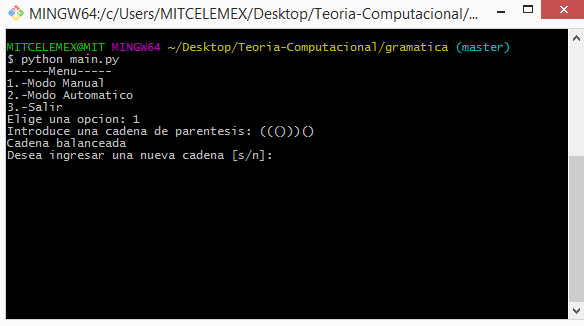
\includegraphics[width=\textwidth, height=7cm]{ModoManualPare.png}
\label{fig:manual_webay}
\caption{Cadena de par\'entesis de prueba: ((()))()}
\end{figure}

\begin{figure}[H]
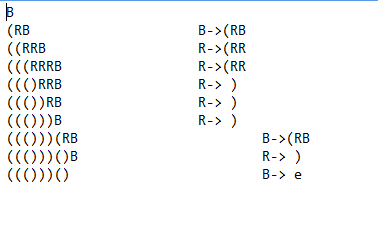
\includegraphics[width=\textwidth, height=7cm]{ArchivoPare.png}
\label{fig:manualtexto_alfabeto}
\caption{Historia de la evaluaci\'on de la cadena}
\end{figure}

Para el modo autom\'atico:\\
\begin{figure}[H]
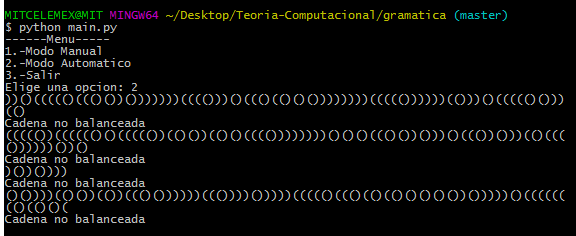
\includegraphics[width=\textwidth, height=7cm]{ModoAutomaticoPare.png}
\label{fig:auto_alfabeto}
\caption{Cadena generada autom\'aticamente}
\end{figure}

\begin{figure}[H]
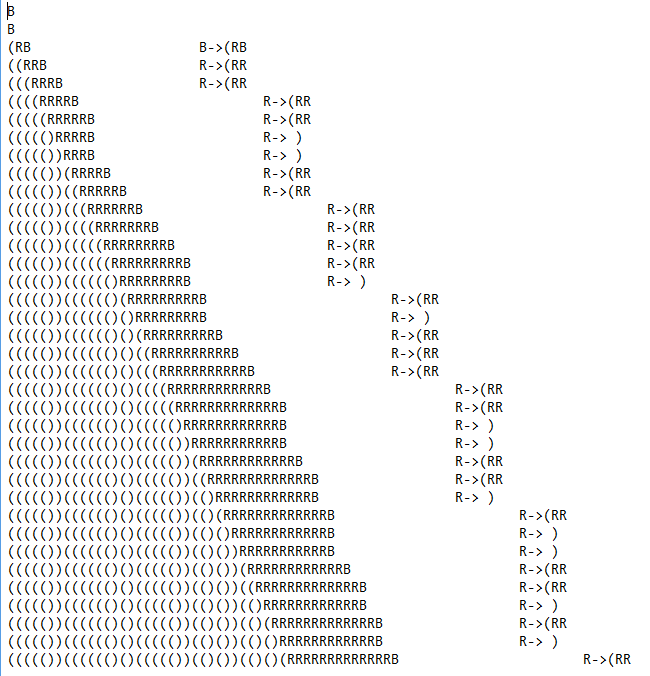
\includegraphics[width=\textwidth, height=7cm]{ArchivoHistoriaPare.png}
\label{fig:autotexto_alfabeto}
\caption{Historia de la evaluaci\'on del modo autom\'atico}
\end{figure}

\newpage
